%%%%%%%%%%%%%%%%%%%%%%%%%%%%%%%%%%%%%%%%%
% Stylish Article
% LaTeX Template
% Version 2.1 (1/10/15)
%
% This template has been downloaded from:
% http://www.LaTeXTemplates.com
%
% Original author:
% Mathias Legrand (legrand.mathias@gmail.com) 
% With extensive modifications by:
% Vel (vel@latextemplates.com)
%
% License:
% CC BY-NC-SA 3.0 (http://creativecommons.org/licenses/by-nc-sa/3.0/)
%
%%%%%%%%%%%%%%%%%%%%%%%%%%%%%%%%%%%%%%%%%

%----------------------------------------------------------------------------------------
%	PACKAGES AND OTHER DOCUMENT CONFIGURATIONS
%----------------------------------------------------------------------------------------

\documentclass[fleqn,12pt]{SelfArx} % Document font size and equations flushed left

\usepackage[english]{babel} % Specify a different language here - english by default

\usepackage{lipsum} % Required to insert dummy text. To be removed otherwise

\captionsetup[figure]{justification=justified, singlelinecheck=off} 
\captionsetup[table]{justification=justified, singlelinecheck=off} 

%----------------------------------------------------------------------------------------
%	COLUMNS
%----------------------------------------------------------------------------------------

\setlength{\columnsep}{0.55cm} % Distance between the two columns of text
\setlength{\fboxrule}{0.75pt} % Width of the border around the abstract
\linespread{1.5}

%----------------------------------------------------------------------------------------
%	COLORS
%----------------------------------------------------------------------------------------

\definecolor{color1}{RGB}{0,0,90} % Color of the article title and sections
\definecolor{color2}{RGB}{10,20,20} % Color of the boxes behind the abstract and headings
\definecolor{xsubj}{RGB}{243,194,68} 
\definecolor{xsess}{RGB}{53,99,161} 
\definecolor{xsamp}{RGB}{18,165,121} 

%----------------------------------------------------------------------------------------
%	HYPERLINKS
%----------------------------------------------------------------------------------------

\usepackage{hyperref} % Required for hyperlinks
\hypersetup{hidelinks,colorlinks,breaklinks=true,urlcolor=color2,citecolor=color1,linkcolor=color1,bookmarksopen=false,pdftitle={Title},pdfauthor={Author}}

%----------------------------------------------------------------------------------------
% Macros that fit better here than the template
%----------------------------------------------------------------------------------------
\makeatletter
\let\Hy@linktoc\Hy@linktoc@none
\let\l@secnonum\l@section
\newcounter{secnonum}
\renewcommand{\thesecnonum}{}
\makeatother

\titleclass{\secnonum}{straight}[\section]
\setcounter{secnumdepth}{3}
\titleformat{\secnonum}
  {}{}{}{}
\titlespacing*{\secnonum}{0pt}{}{}
\newcommand{\secnonumautorefname}{secnonum}

%----------------------------------------------------------------------------------------
%	ARTICLE INFORMATION
%----------------------------------------------------------------------------------------

% \JournalInfo{Journal, Vol. XXI, No. 1, 1-5, 2013} % Journal information
\JournalInfo{$ $ } % Journal information
\Archive{Ph.D. Thesis} % Additional notes (e.g. copyright, DOI, review/research article)

\PaperTitle{This is Your Brain on Disk: The Impact of Numerical Instabilities in Neuroscience} % Article title

\Authors{Gregory Kiar\textsuperscript{1}, Alan C. Evans\textsuperscript{1$\dagger$}, Tristan Glatard\textsuperscript{2$\dagger$}} % Authors
\affiliation{\textsuperscript{1}\textit{Montréal Neurological Institute, McGill University, Montréal, QC, Canada}}
\affiliation{\textsuperscript{2}\textit{Department of Computer Science and Software Engineering, Concordia University, Montréal, QC, Canada}}

\Keywords{Stability --- Reproducibility --- Network Neuroscience --- Neuroimaging} % Keywords - if you don't want any simply remove all the text between the curly brackets
\newcommand{\keywordname}{Keywords} % Defines the keywords heading name

%----------------------------------------------------------------------------------------
%	ABSTRACT
%----------------------------------------------------------------------------------------

\Abstract{blnk}

%----------------------------------------------------------------------------------------

\begin{document}

\flushbottom % Makes all text pages the same height
\maketitle % Print the title and abstract box
\onecolumn
\tableofcontents % Print the contents section
\twocolumn

\phantomsection
\section{intro}
words

\phantomsection
\section{bg}
hithere

\thispagestyle{empty} % Removes page numbering from the first page

%----------------------------------------------------------------------------------------
%	ARTICLE CONTENTS
%----------------------------------------------------------------------------------------
\onecolumn
\clearpage

\phantomsection
\beginchapter{I}
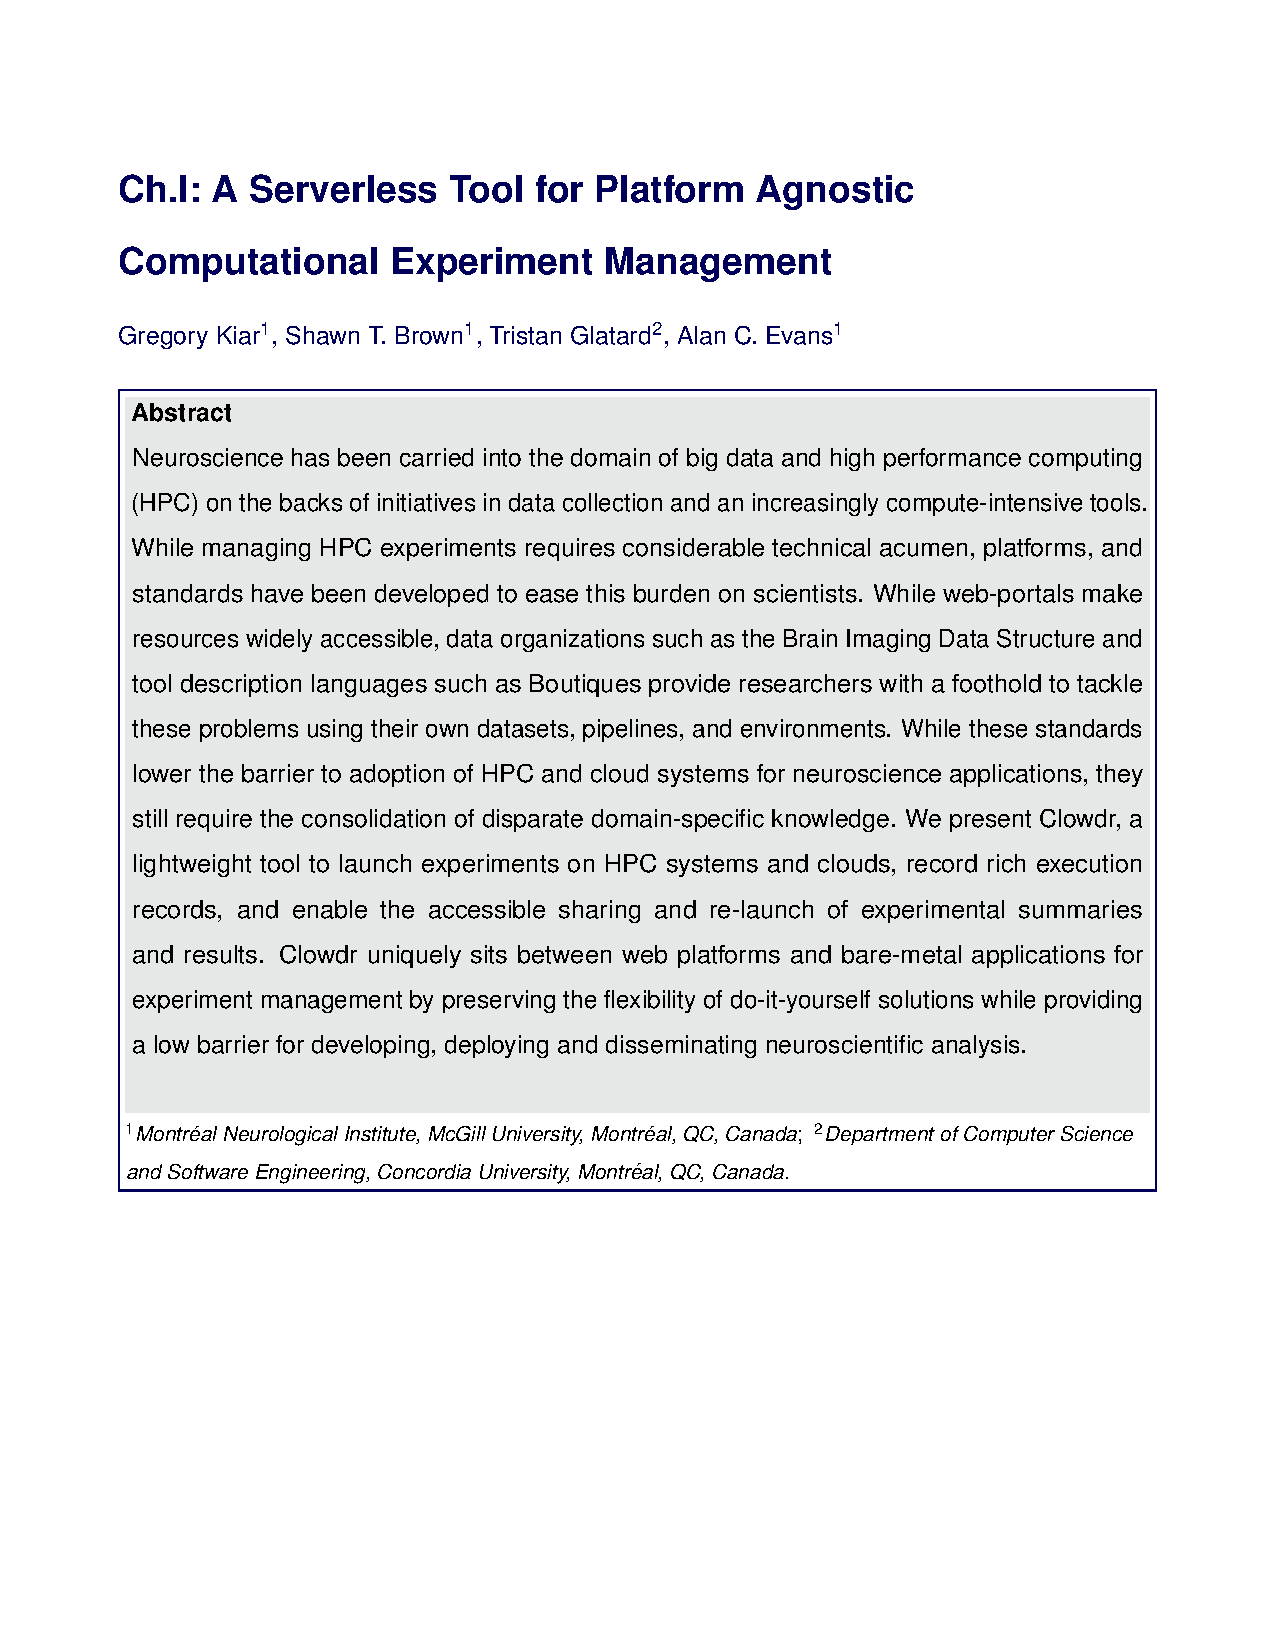
\includepdf[pages=-,pagecommand={\thispagestyle{fancy}},addtotoc={
     1,part,1,A Serverless Tool for Platform Agnostic Computational Experiment Management,ch1p1,   
     1,secnonum,2,Abstract,ch1p2,
     2,section,2,Introduction,ch1p2,
     3,section,2,Emergent Technologies in Reproducible Neuroscience,ch1p3,
     3,section,2,Emergent Technologies in Reproducible Neuroscience,ch1p3,
     6,section,2,The Clowdr Microtool,ch1p6,
     9,section,2,Performing Experiments With Clowdr,ch1p9,
     12,section,2,Discussion,ch1p12}]
     {../chapter1/chapter1.pdf}
\clearpage

\phantomsection
\beginchapter{II}
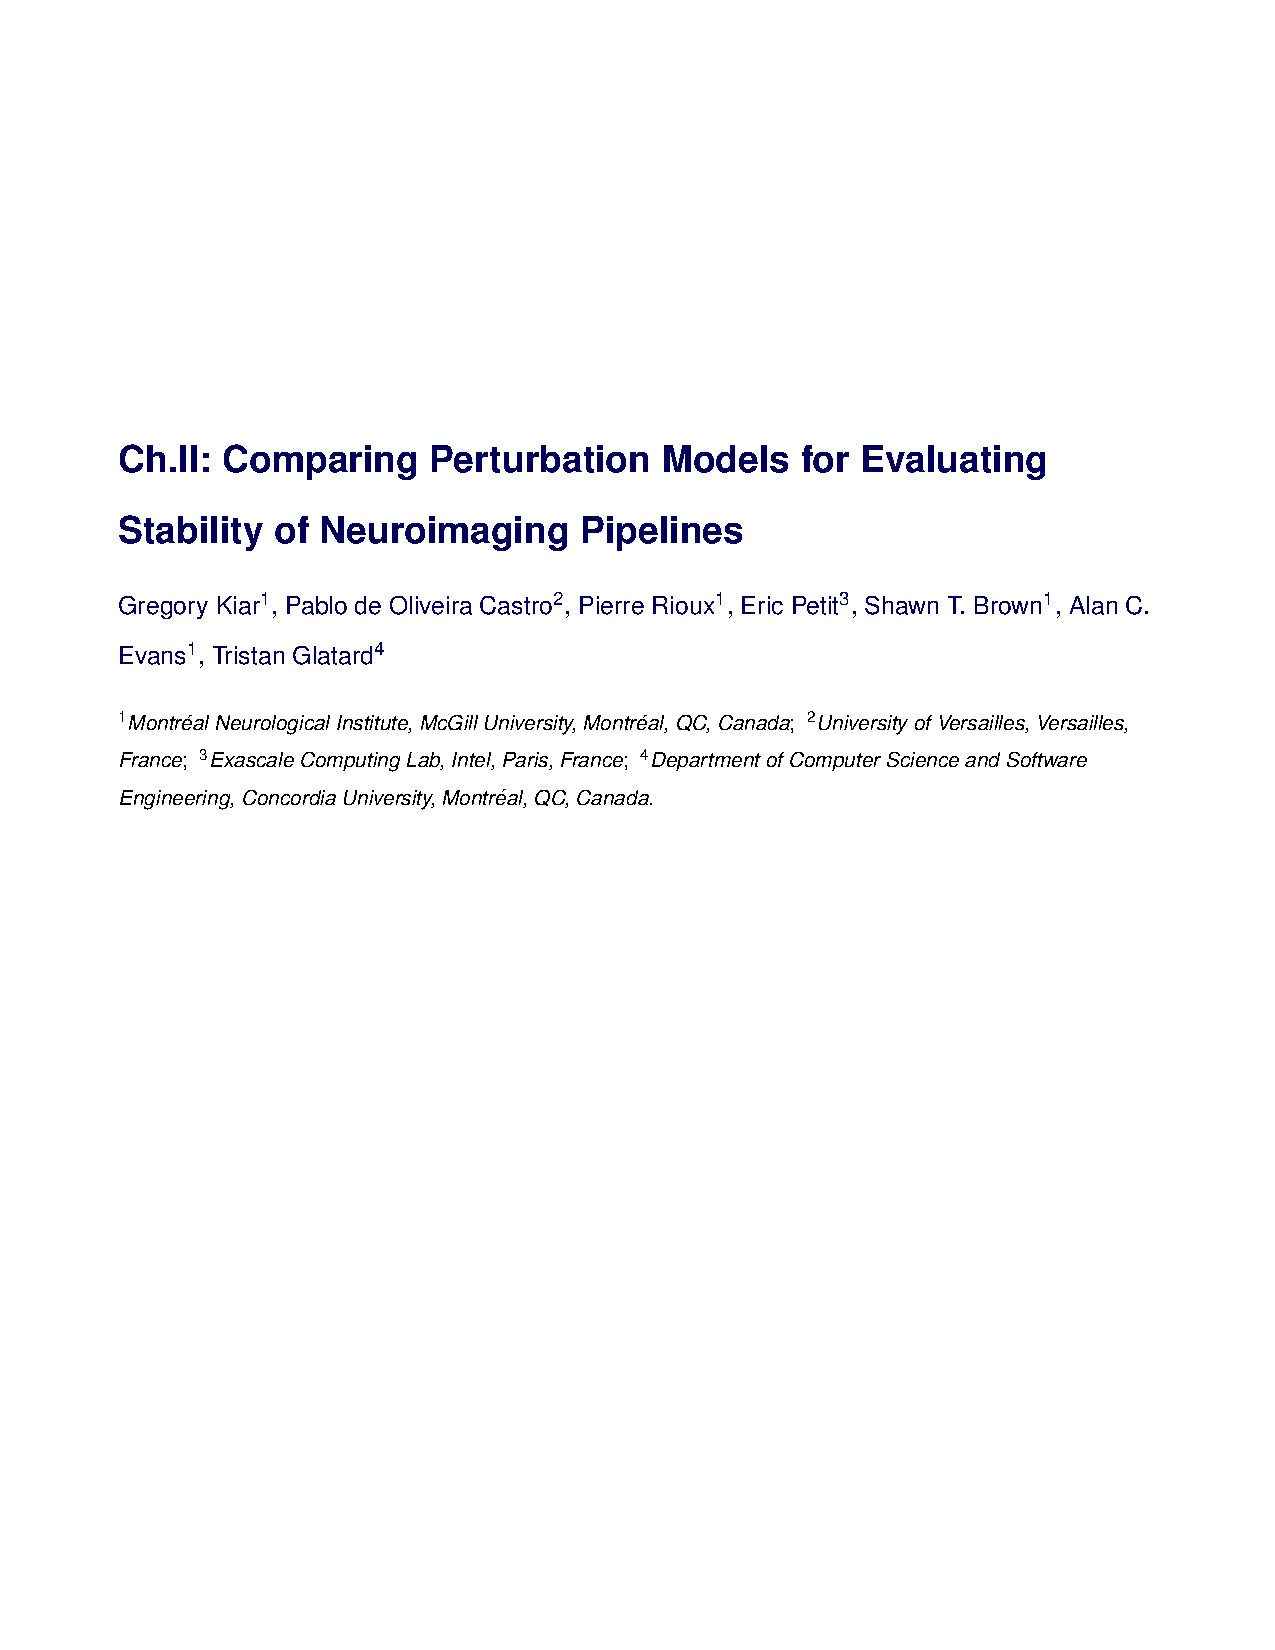
\includepdf[pages=-,addtotoc={
     1,part,1,Comparing Perturbation Models for Evaluating Stability of Neuroimaging Pipelines,ch2p1,   
     1,section,2,Subsection Entry,ch2p2,
     2,section,3,Second Section Entry,ch2p3}]
     {../chapter2/chapter2.pdf}
\clearpage

\phantomsection
\beginchapter{III}
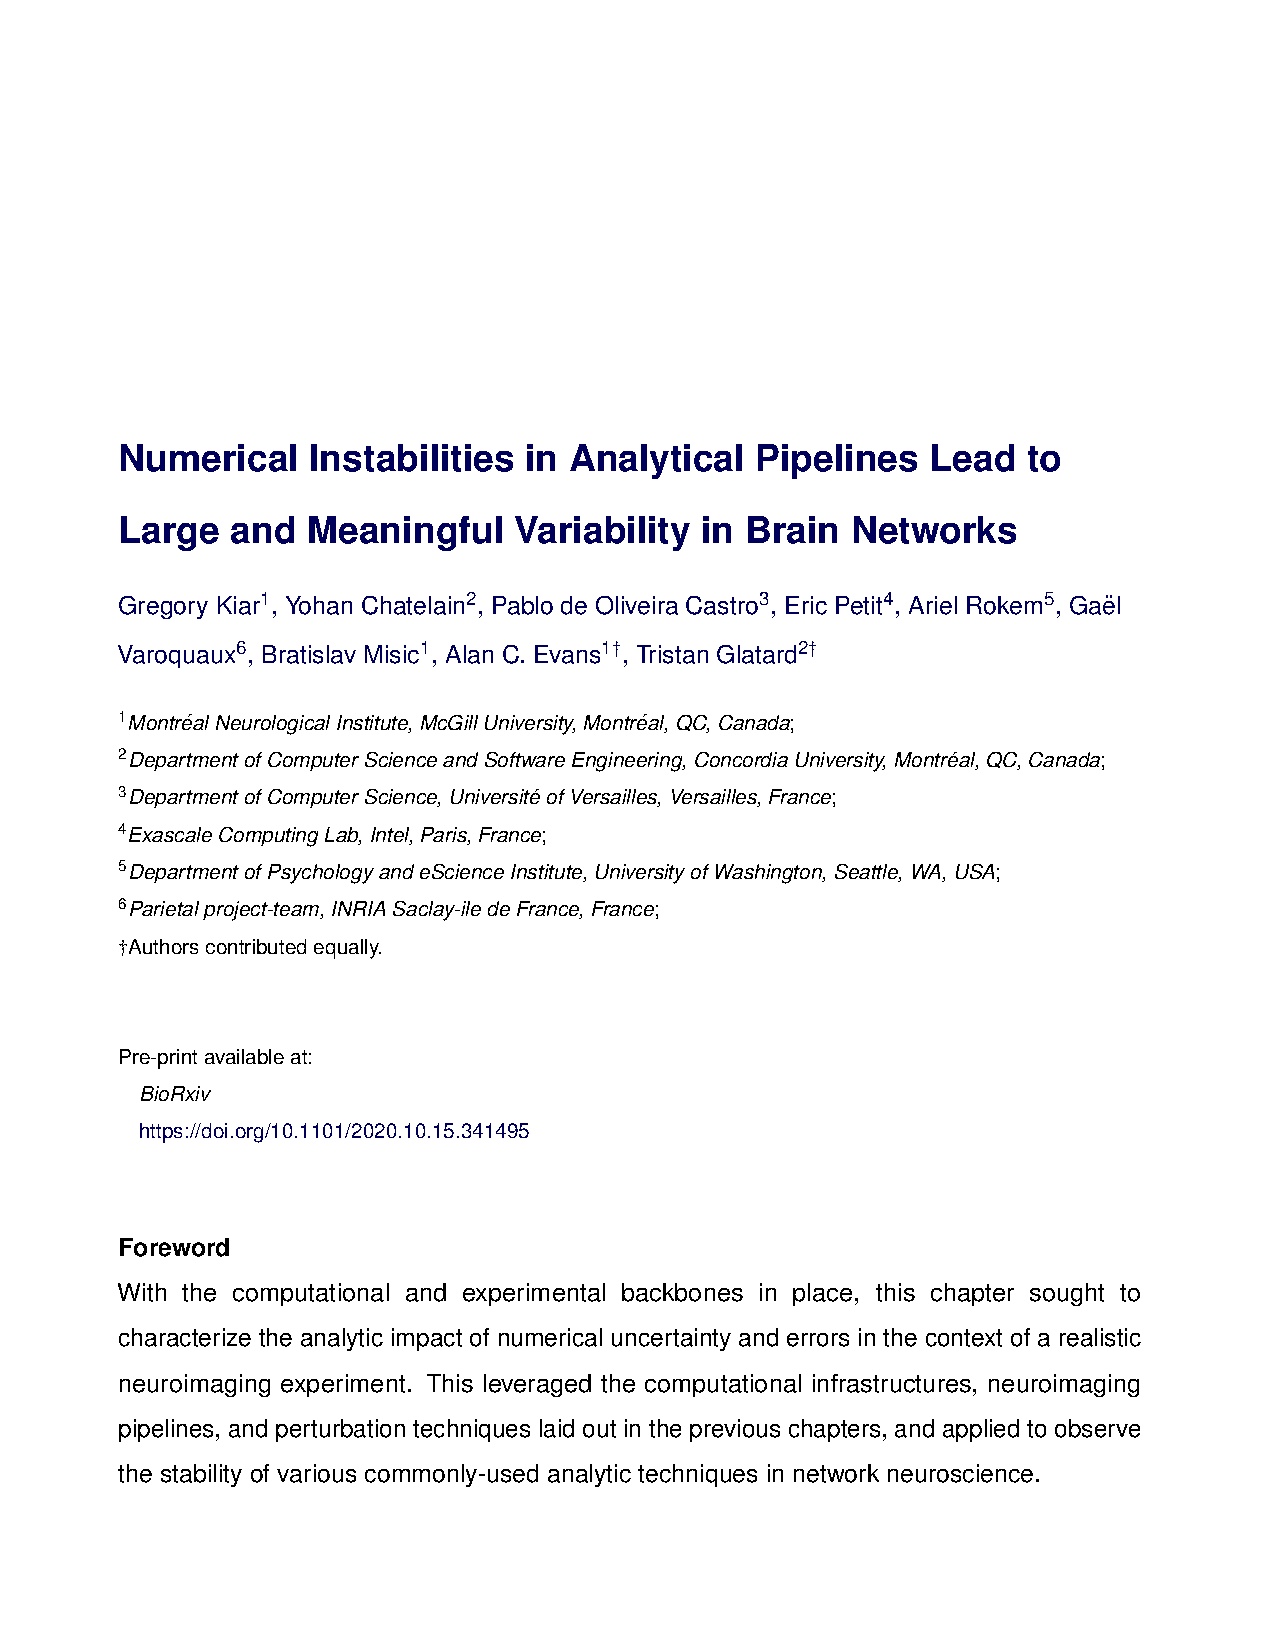
\includepdf[pages=-,addtotoc={
     1,part,1,Numerical Instabilities in Analytical Pipelines Lead to Large and Meaningful \\ Variability in Brain Networks,ch3p1,   
     1,subsection,2,Subsection Entry,ch3p2,
     2,subsection,3,Second Section Entry,ch3p3}]
     {../chapter3/chapter3.pdf}
\twocolumn

\resetsections{2}
\phantomsection
\section{discus}
hi there

%----------------------------------------------------------------------------------------
%	REFERENCE LIST
%----------------------------------------------------------------------------------------
% \phantomsection
% \bibliographystyle{IEEEtran}
% \bibliography{gkiar_thesis}

%----------------------------------------------------------------------------------------
\end{document}
